\section{Limitations and Future Work}\label{sec:limitations}

A promising direction for future work is extending SCONE beyond short $n$-grams by enabling caching for longer queries. A central challenge lies in designing effective keys for such queries. Using raw text as keys may result in low cache hit rates, as semantically similar queries often vary at the surface level. Alternatively, using semantic embeddings as keys would require discretization techniques to map continuous embeddings into a discrete key space that supports efficient indexing.

One limitation of the current study is that we evaluate SCONE only on models with up to 3B parameters at training time. This constraint is primarily due to hardware limitations, which restrict our ability to conduct large-scale pretraining on larger models. Although the model scales we tested are widely used in real-world applications, exploring the performance of SCONE at larger scales presents an exciting direction for future research. We believe applying SCONE to larger models would be highly beneficial to the community and leave this exploration for future work. Notably, our experiments in \Cref{sec:exps_openwebtext} provide encouraging evidence, as the benefits of SCONE are consistent across all model sizes we tested.

\section{Additional Related Work}\label{sec:add_related_work}

\paragraph{Contextualized Word Embeddings.} Words can have different meanings depending on context. Prior work has incorporated context into word embeddings, either from the entire sequence \citep{mccann2017learned,peters2018deep} or short \ngram{n}s \citep{gupta2019better}, before applying them to downstream tasks. Modern language models inherently use contextualized token embeddings, leveraging attention mechanisms. In this study, we extend the embedding layer to include contextualized f-gram embeddings for each token. A key novelty is that our approach allows embeddings to be precomputed and offloaded from accelerators, providing contextual embeddings for each token without increasing FLOPS and accelerator memory usage at inference.


\paragraph{Tokenization in Language Models.} Our method assumes a predefined vocabulary from a trained tokenizer. Several popular algorithms exist for training tokenizers \citep{sennrich2015neural, wu2016google, kudo2018subword, kudo2018sentencepiece}. In this work, we use a BPE tokenizer, following prior seminal works \citep{radford2019language, touvron2023llama}. However, our method is not tied to any specific tokenization algorithm and can be applied seamlessly to others.

Tokenization-free language models have also been widely explored \citep{kim2016character, choe2019bridging, xue2022byt5, yu2023megabyte, wang2024mambabyte, deiseroth2024t, meta2024large, pagnoni2024byte}. While we have not tested our method on tokenization-free models, we believe our core idea—introducing an off-accelerator embedding layer by precomputing embeddings for frequent input patterns—remains applicable.



\paragraph{Mixture-of-Experts (MoE) and Memory Layers.} MoE and memory layers are two established approaches for scaling language models within a fixed FLOPS budget.

MoE layers replace traditional feedforward layers with multiple parallel ``experts," activating only one or a few per token using a lightweight routing mechanism \citep{shazeer2017outrageously,lepikhin2021gshard,fedus2022switch,jiang2024mixtral,he2024mixture}. This allows the model to scale by increasing the number of experts without increasing the computational cost per token. However, all experts must reside on the accelerator, resulting in significantly higher memory usage.

Memory layers, on the other hand, store large collections of embeddings (continuous vectors) and retrieve the nearest neighbors during the forward pass via (approximate) similarity search \citep{weston2014memory,sukhbaatar2015end,lample2019large,berges2024memory}. These retrieved embeddings enhance the model’s capabilities without adding much to the FLOPS budget. Despite improvements in similarity search techniques \citep{lample2019large,johnson2019billion}, memory layers still require storing the embeddings on the accelerator, making memory demands impractically high at larger scales \citep{berges2024memory}. Furthermore, because embeddings are typically updated via backpropagation, memory layers introduce additional challenges related to sparse updates as the memory size grows.

While MoE layers, memory layers, and our proposed method \SCONE all maintain fixed inference FLOPS, a key advantage of \SCONE is it also maintains fixed accelerator memory usage at inference. By focusing on the input embedding layer, \SCONE ensures that the computational overhead remains $O(1)$ during inference and enables offloading the additional parameters off-accelerator with negligible impact on end-to-end latency.



\paragraph{Implicit $n$-gram Patterns in Transformers.} Recent work analyzing the internal mechanisms of transformers has shown that these models often utilize implicit $n$-gram patterns for prediction \citep{geva2020transformer,geva2022transformer,voita2023neurons}. For instance, \citet{chen2024jet} demonstrate that certain attention heads can detect specific $n$-gram patterns, while MLPs can perform linguistic operations such as adding the “-ing” suffix. These findings underscore the importance of $n$-gram information in language modeling and offer a potential explanation for the effectiveness of \SCONE. An interesting future direction is to examine how \SCONE's f-gram embeddings interact with the transformer’s implicit $n$-gram patterns.

\paragraph{Embedding Sparsity in Multilingual Applications and Recommender Systems.} This work focuses on a common setting for training LLMs: language modeling on large-scale text corpora, primarily in English. However, scaling embedding layers presents challenges beyond this context, particularly due to frequency-related performance degradation caused by sparsity. Multilingual applications are one such scenario. Two phrases in different languages may refer to the same concept but correspond to different embedding vectors. Their embeddings should ideally be close. Recent work has explored methods for learning transferable embeddings in cross-lingual settings \citep{artetxe2019cross, chen2023improving}. Another relevant example is scaling the embeddings for recommender systems \citep{chen2019lambdaopt, liu2021learnable}, where embeddings often dominate the model's parameter count due to the high cardinality of user or item categories. For both scenarios, \SCONE’s strategy, i.e., parameterizing large embedding tables using a neural network, provides a complementary approach to help mitigate sparsity issues.

\section{Additional Algorithms}\label{sec:add_algorithms}



{\renewcommand{\baselinestretch}{1.35}\selectfont
\begin{algorithm}[t]
\caption{Basic Next-Word Prediction Model $M_{\cT, \cA, \cD}$.}
\label{alg:basic-model}
\begin{algorithmic}
\STATE {\bf Parameters:}\begin{itemize}[itemsep=-3pt]
    \item $\cT : \Vtoken \to \R^d$: token embedding layer,
    \item $\cA : (\R^d)^{\le T} \to \R^d$: transformer model, where $T$ is the maximum sequence length,
    \item $\cD : \R^d \to \Delta_{\Vtoken}$: prediction head.
\end{itemize}
\STATE {\bf Input:} $(\sigma_1, \ldots, \sigma_m) \in \Vtoken^*$ for $m \le T$.
\STATE {\bf Output:} Probability distribution over next token $\hat{\sigma}_{m+1}$.
\FOR{$i=1, \ldots, m$}
    \STATE $\be_i \gets \cT(\sigma_i)$ : Input embedding per token.
\ENDFOR
\STATE $\be_{\mathrm{out}} \gets \cA(\be_1, \ldots, \be_m)$: Output embedding.
\RETURN $D(\be_{\mathrm{out}})$
\end{algorithmic}
\end{algorithm}
}


{\renewcommand{\baselinestretch}{1.35}\selectfont
\begin{algorithm}[t]
\caption{Constructing a set of f-grams $\Vfgram$.}
\label{alg:n-gram-vocab}
\begin{algorithmic}
\STATE {\bf Parameters:} $S$: desired size of $\Vfgram$.
\STATE {\bf Input:} $\{(\sigma_1, \ldots, \sigma_{T})^{(i)}\}$ : token sequences from training set.
\STATE {\bf Output:} $\Vfgram \subseteq \Vtoken^{[2,K]}$: set of f-grams of size $S$.
\FOR{$n = 2, \ldots, K$}
    \FOR{$\omega := (\sigma^{'}_1, \ldots, \sigma^{'}_k) \in \Vtoken^{n}$}
        \STATE $C_{\omega} \gets$ the number of times $\omega$ appears in all sequences $\{(\sigma_1, \ldots, \sigma_{T})^{(i)}\}$.
    \ENDFOR
\ENDFOR
\STATE Let $\omega_1, \omega_2, \ldots $ be list of elements of $\bigcup_{n=2}^K \Vtoken^{n}$, sorted such that $C_{\omega_1} \ge C_{\omega_2} \ge \cdots$, breaking ties arbitrarily.
\RETURN $\{\omega_1, \ldots, \omega_{S}\}$: set of f-grams of size $S$.
\end{algorithmic}
\end{algorithm}
}

{\renewcommand{\baselinestretch}{1.35}\selectfont
\begin{algorithm}[h]
\caption{Next-word prediction with \SCONE  $M_{\cT, \Vfgram, \train{\Afgram}|\infer{\cF}, \Amain, \cD}$}
\label{alg:scone-model}
\begin{algorithmic}
\STATE {\bf Parameters:}\begin{itemize}[itemsep=-3pt]
    \item $\cT : \Vtoken \to \R^d$: token embedding layer,
    \item $\Vfgram \subseteq \Vtoken^{[2,K]}$: set of f-grams,
    \item \textbf{\textsc{Training}}: f-gram transformer model
    \begin{itemize}[leftmargin=8mm,label=$\triangleright$,itemsep=-3pt,topsep=-4pt]
        \item \train{$\Afgram : (\R^d)^{\le K} \to \R^d$},
    \end{itemize}
    \item \textbf{\textsc{Inference}}: f-gram embedding layer
    \begin{itemize}[leftmargin=8mm,label=$\triangleright$,itemsep=-3pt,topsep=-4pt]
        \item \infer{$\cF : \Vfgram \to \R^d$}.
    \end{itemize}
    \item $\Amain : (\R^d)^{\le T} \to \R^d$: main transformer model.
    \item $\cD : \R^d \to \Delta_{\Vtoken}$: Prediction head.
\end{itemize}
\STATE {\bf Input:} $(\sigma_1, \ldots, \sigma_m) \in \Vtoken^*$ for $m \le T$, where $T$ is the maximum sequence length.
\STATE {\bf Output:} Probability distribution over next token $\hat{\sigma}_{m+1}$.
\STATE $(\be_1, \ldots, \be_m) \gets F_{\cT, \Vfgram, \train{\Afgram} | \infer{\cF}}(\sigma_1, \ldots, \sigma_m)$ (\Cref{alg:scone-first-stage})
\STATE $\be_{\mathrm{out}} \gets \Amain(\be_1, \ldots, \be_m)$
\RETURN $D(\be_{\mathrm{out}})$
\end{algorithmic}
\end{algorithm}
}

In \Cref{sec:preliminary}, we discuss a simple next-word prediction model, \( M_{\cT, \cA, \cD} \), consisting of a token embedding layer \( \cT \), a transformer model \( \cA \), and a prediction head \( \cD \). This model takes a token sequence \( (\sigma_1, \ldots, \sigma_m) \), with each token from the token vocabulary \( \Vtoken \), and produces a probability distribution for the next token. We provide the pseudocode for \( M_{\cT, \cA, \cD} \) in \Cref{alg:basic-model}.

In \Cref{sec:method}, we introduce an algorithm for constructing a set of f-grams given a target number of f-grams. We present the pseudocode for the construction process in \Cref{alg:n-gram-vocab}. Although \Cref{alg:n-gram-vocab} clearly illustrates the procedure, it is too expensive to implement in practice. In \Cref{subsec:key_discovery}, we describe an efficient implementation that requires only $K-1$ linear scans over the pre-training corpus, where $K$ is a hyperparameter controlling the maximum length of f-grams.




In \Cref{alg:scone-first-stage} in \Cref{sec:method}, we present the pseudocode for \SCONE's process of generating contextualized f-gram embeddings. Next, we describe the end-to-end next-word prediction process using \SCONE (\Cref{alg:scone-model}). Specifically, the process, denoted as $M_{\cT, \Vfgram, \train{\Afgram} | \infer{\cF}, \Amain, \cD}$, takes an input sequence $(\sigma_1, \ldots, \sigma_m) \in \Vtoken^*$ and produces a distribution over the next token $\hat{\sigma}_{m+1}$. Note that in \Cref{alg:scone-model}, f-gram embeddings are generated with $\Afgram$ during training and retrieved from a lookup table $\cF$ during inference.



\section{Challenges of Scaling Vocabulary Size in Embedding Layers}
\label{sec:scale_vocab}

Scaling the token vocabulary size is the most straightforward way to enlarge an embedding layer, but we find that larger token vocabularies degrade performance beyond a certain threshold and significantly increase accelerator usage during decoding. We pre-train GPT-2 models \citep{radford2019language} with three sizes of non-embedding parameters: 85M (small), 302M (medium), and 708M (large) on the WebText dataset \citep{openwebtext}, testing six vocabulary sizes ranging from 32,768 to 2,097,152. The tokenizers are trained using the BPE algorithm \citep{gage1994new, sennrich2015neural}. We follow the implementation in \citet{tao2024scaling}, which allows token merges across word boundaries. Each model is trained on 80B tokens. Since larger vocabularies produce fewer tokens for the same dataset, they effectively enable models to process more data. Additional implementation details such as training hyperparameters are provided in Appendix~\ref{subsec:webtext_details}.

\begin{figure}[h]
    \centering
    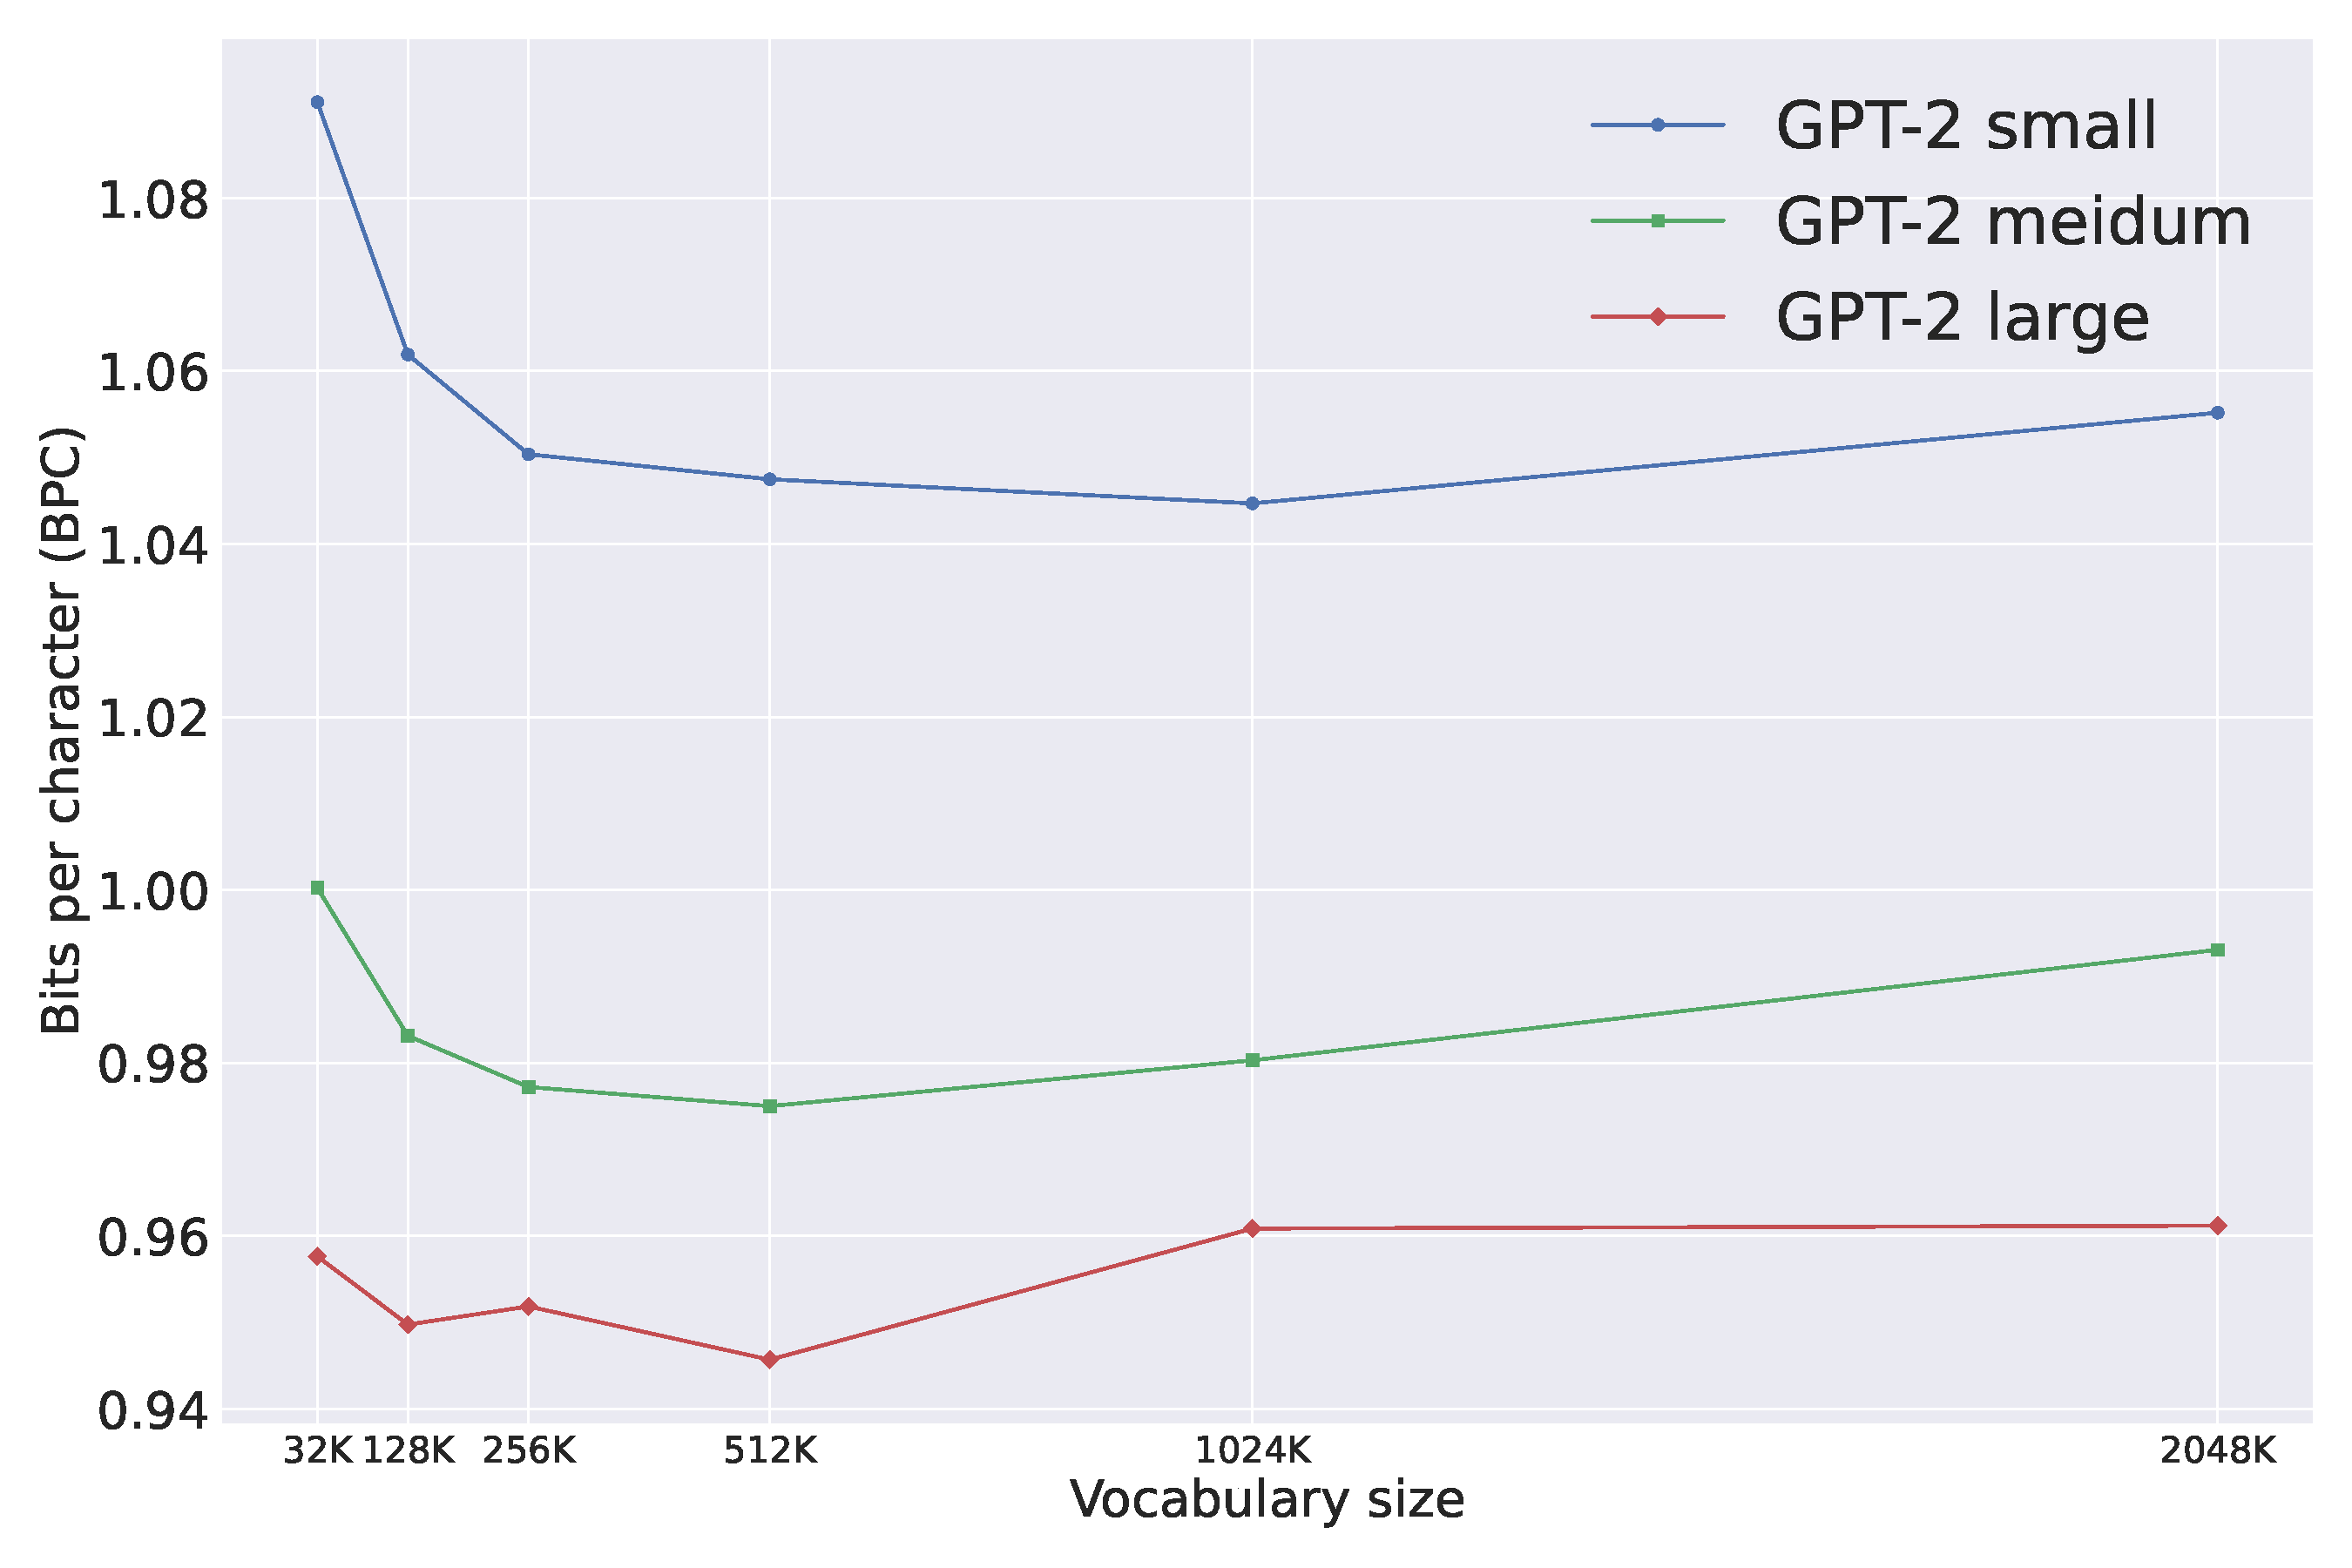
\includegraphics[width=0.45\linewidth]{figs/openwebtext_vocab_size_bpc_loss.pdf}
    \caption{BPC of three model sizes on the validation set (lower is better). For all three model sizes, BPC initially improves as vocabulary size increases but eventually deteriorates.}
    \label{fig:bpc_vary_vocab}
\end{figure}

Figure~\ref{fig:bpc_vary_vocab} presents the average bits per character (BPC) on the WebText validation set. We report BPC instead of cross-entropy loss because the latter is sensitive to vocabulary size, with larger vocabularies typically producing higher losses. BPC, by contrast, is a common vocabulary-insensitive metric for comparing models trained with different tokenizers \citep{huang2024compression}. We observe that BPC for all three models initially improves with larger vocabulary sizes but eventually deteriorates.


\begin{figure}[h]
    \centering
    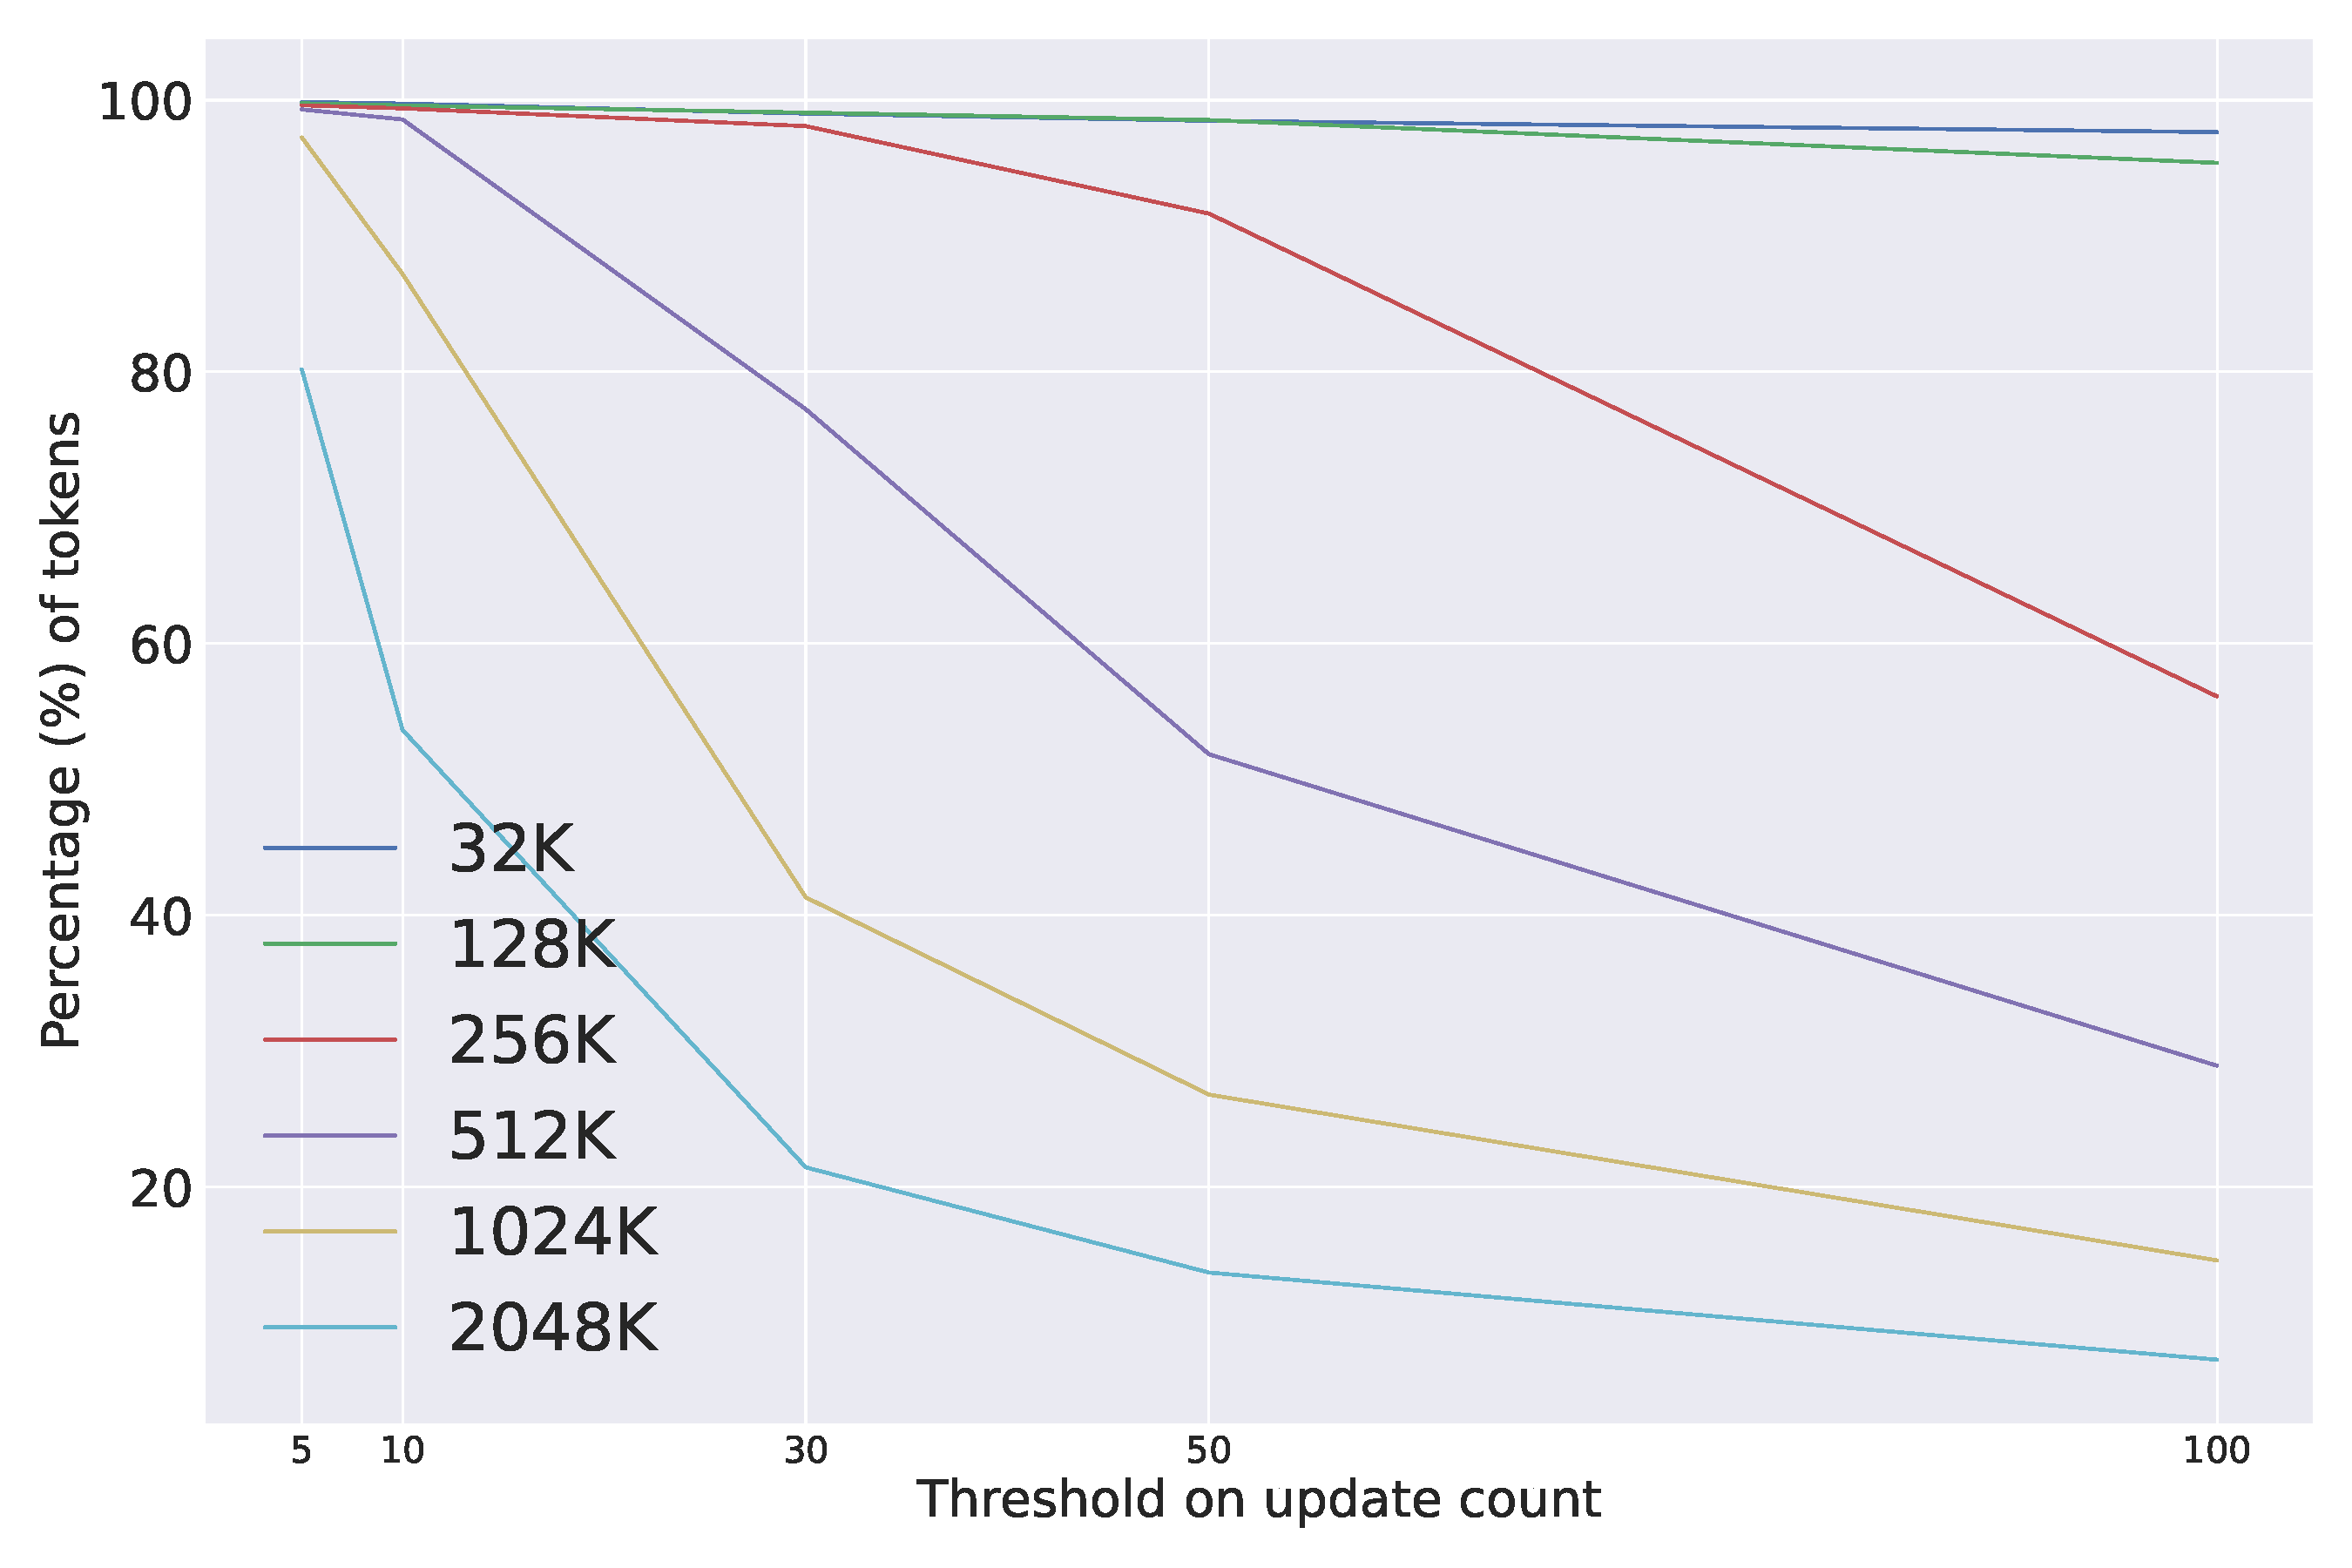
\includegraphics[width=0.45\linewidth]{figs/openwebtext_vocab_size_update_freq.pdf}
    \caption{Percentages of tokens ($y$-axis) that receive more than a given number of updates ($x$-axis), measured over 100M training tokens. As the vocabulary size increases, tokens receive increasingly sparse updates.}
    \label{fig:update_freq_vary_vocab}
\end{figure}


Figure~\ref{fig:update_freq_vary_vocab} shows the percentages  of tokens that receive more than a given number of updates over 100M training tokens. In standard embedding layers, gradients are directly backpropagated to the embedding vectors. With a fixed number of training tokens, larger vocabularies lead to fewer updates per token. For a vocabulary size of 2,097,152, only 7.3\% of tokens receive more than 100 updates, compared to 97.6\% for a vocabulary size of 32,768. This suggests that the performance drop for larger vocabularies may stem from sparse updates to per-token embedding vectors.

\begin{figure}[h]
    \centering
    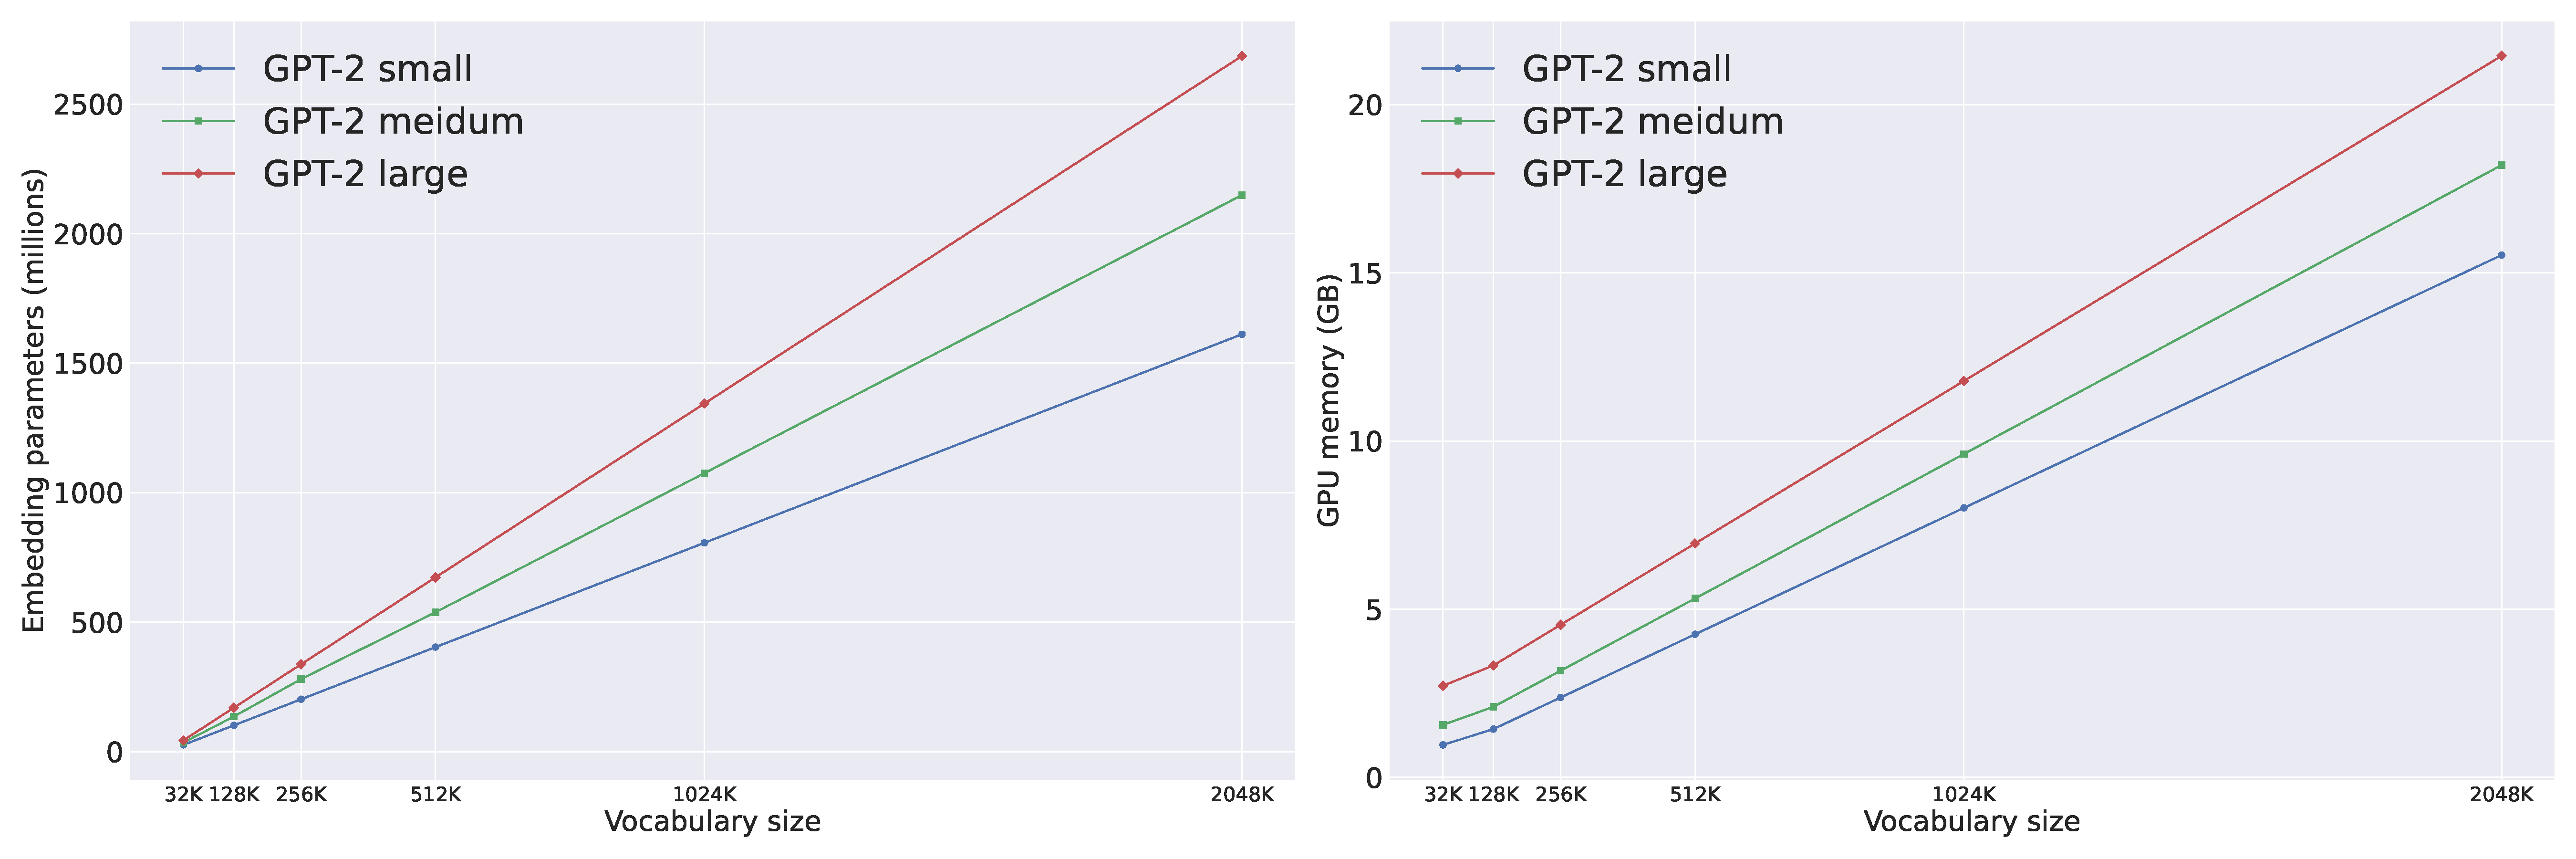
\includegraphics[width=1.0\linewidth]{figs/openwebtext_vocab_size_params_memory.pdf}
    \caption{Number of embedding layer parameters stored on GPU and the corresponding memory usage. For large vocabulary sizes, the memory usage increases linearly with the vocabulary size.}
    \label{fig:gpu_cost_vary_vocab}
\end{figure}



In addition to performance degradation, increasing the vocabulary size significantly raises accelerator usage during the inference stage. This is because predicting the next token involves running a linear layer and softmax operation across the entire vocabulary to identify the closest embedding. Figure~\ref{fig:gpu_cost_vary_vocab} illustrates that both the number of embedding layer parameters stored on the GPU and the GPU memory cost increase linearly with vocabulary size. These costs are measured using a batch size of 1, a sequence length of 1024, and 16-bit precision. 








\section{Additional Experiments}
\label{sec:addition_results}

\subsection{More Results for Training on WebText}
\label{subsec:more_exp_webtext}

\begin{figure}
\centering
\begin{minipage}{.46\textwidth}
  \centering
  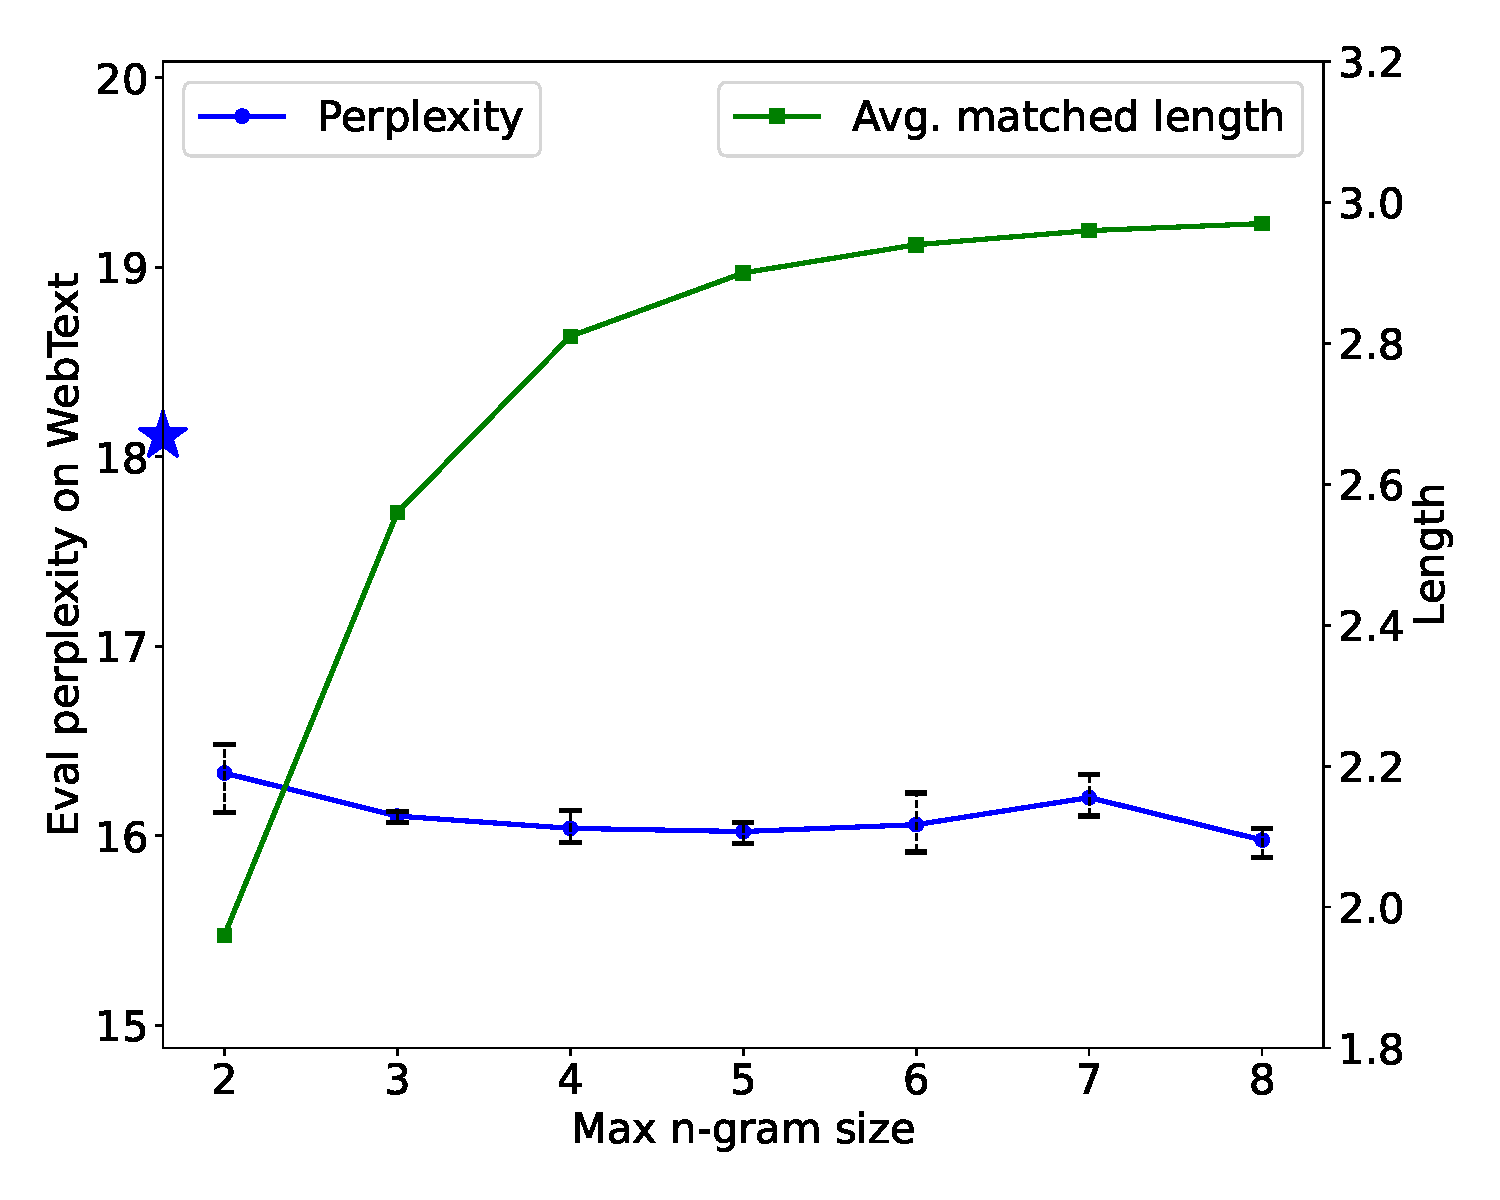
\includegraphics[width=.95\linewidth]{figs/openwebtext_maxngramsize_eval_loss_WebText.pdf}
  \captionof{figure}{Effect of the maximum f-gram length in $\Vfgram$, evaluated on the WebText validation split. }
  \label{fig:scale_max_ngram_size_appendix}
\end{minipage}%
\hspace{0.05\textwidth}
\begin{minipage}{.46\textwidth}
  \centering
  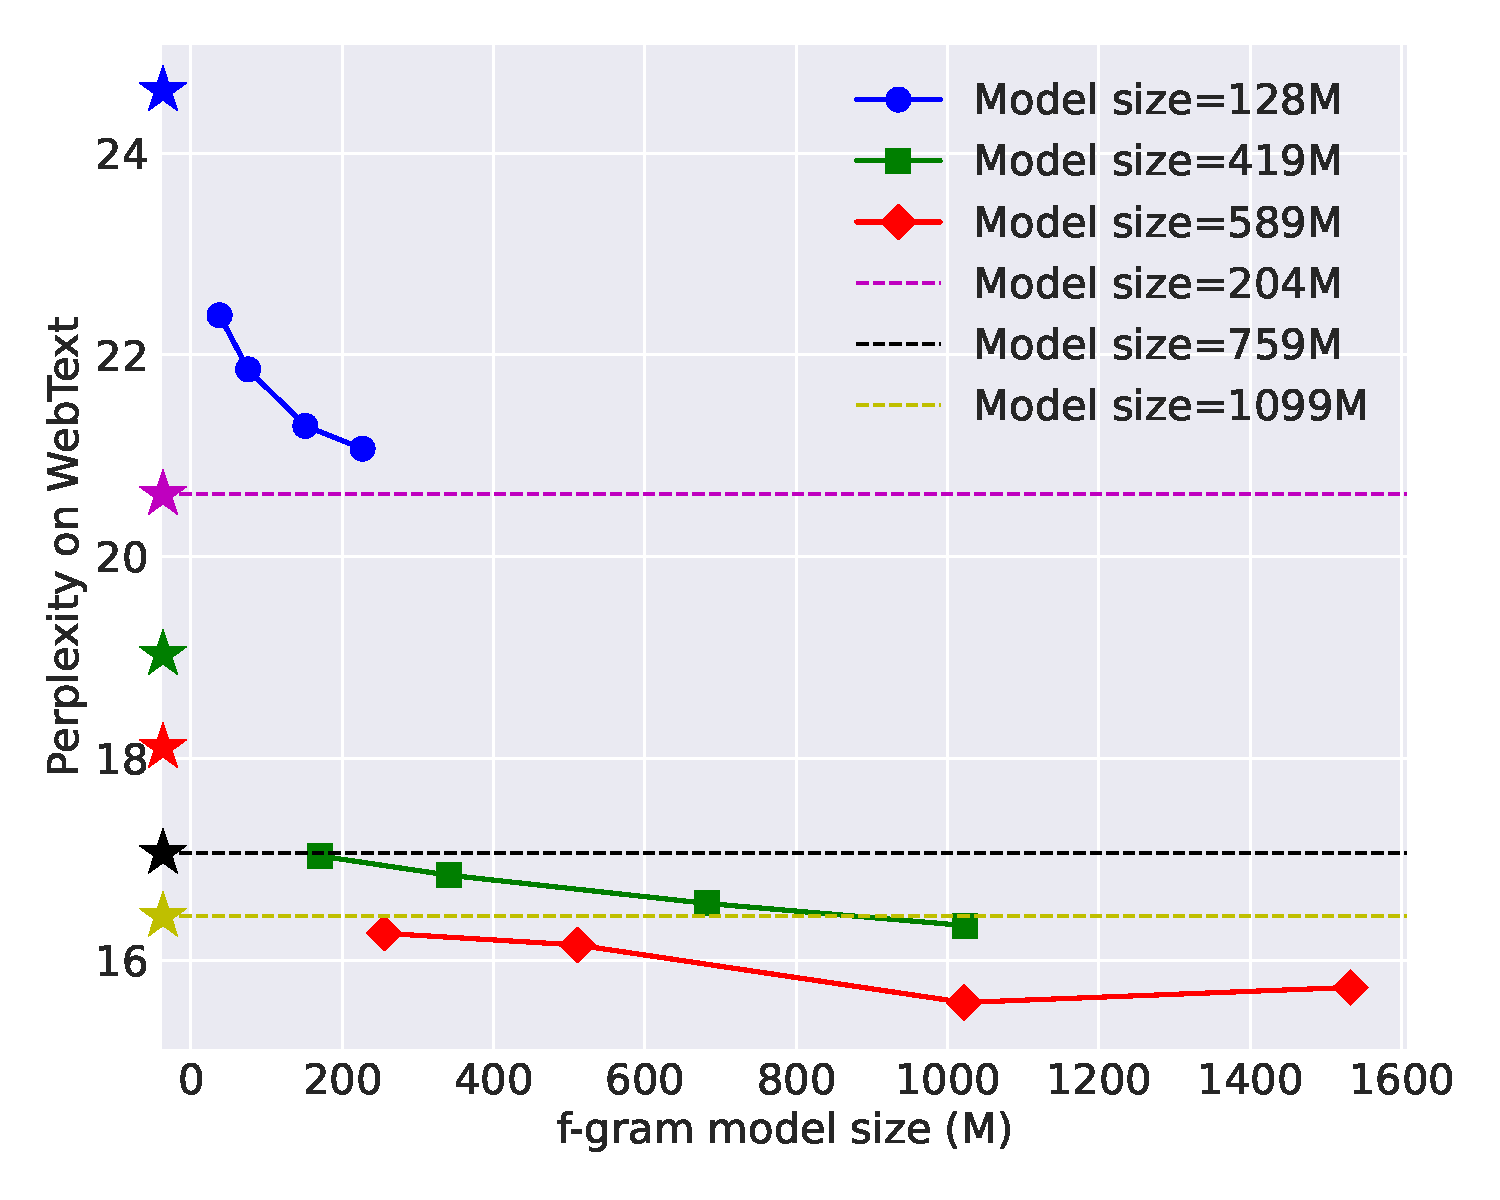
\includegraphics[width=.93\linewidth]{figs/openwebtext_ngrammodel_size_eval_loss_WebText.pdf}
  \captionof{figure}{Evaluation perplexity on WebText as a function of the size of $\Afgram$.}
  \label{fig:scale_ngram_model_appendix}
\end{minipage}
\end{figure}

\paragraph{\boldmath Varying Maximum f-gram Length.}  In \Cref{subsec:max_ngram_size}, we discuss the impact of varying the maximum f-gram length in $\Vfgram$ and present results on Wikitext-103. We observe that a relatively small maximum length is sufficient, as long as it is not too small, otherwise, the number of available \ngram{n}s for ranking becomes too limited. Here, in \Cref{fig:scale_max_ngram_size_appendix}, we show the corresponding results on WebText, which exhibit similar trends. The left $y$-axis represents the evaluation loss (averaged over three seeds), with the leftmost star indicating baseline performance. The right $y$-axis shows the average length of matched f-grams. As the maximum size increases, the loss initially decreases but then plateaus with some fluctuations. Meanwhile, the matched length rises initially before stabilizing for larger values. 

\paragraph{\boldmath Varying $\Afgram$ Model Size.} In \Cref{subsec:ngram_model_size}, we discuss the impact of varying the size of $\Afgram$ on evaluation perplexity for Wikitext-103. We find that increasing the model size leads to further performance improvements for a fixed $|\Vfgram|$. In \Cref{fig:scale_ngram_model_appendix}, we present the results on WebText, which show a similar trend. Model sizes in the legend correspond to inference-time sizes on accelerators. Dashed lines and stars on the left represent baseline performance.  The evaluation perplexity improves as the size of $\Afgram$ grows.




\subsection{Additional Results for Training on the OLMo Corpus}
\label{subsec:more_exp_dolma}

We present training curves and perplexity evaluations for models trained on the OLMo corpus. For \SCONE, we introduce an additional $\Afgram$ model size of 0.6B, alongside the 1.8B $\Afgram$ model discussed in \Cref{sec:exps_dolma}. Due to the large number of experiments, all models in this section are trained for 200B tokens, constrained by computational resources. This differs from \Cref{sec:exps_dolma}, where \SCONE-enabled models are trained for 500B tokens and baseline models for 1T tokens.

\begin{figure}[!h]
    \centering
    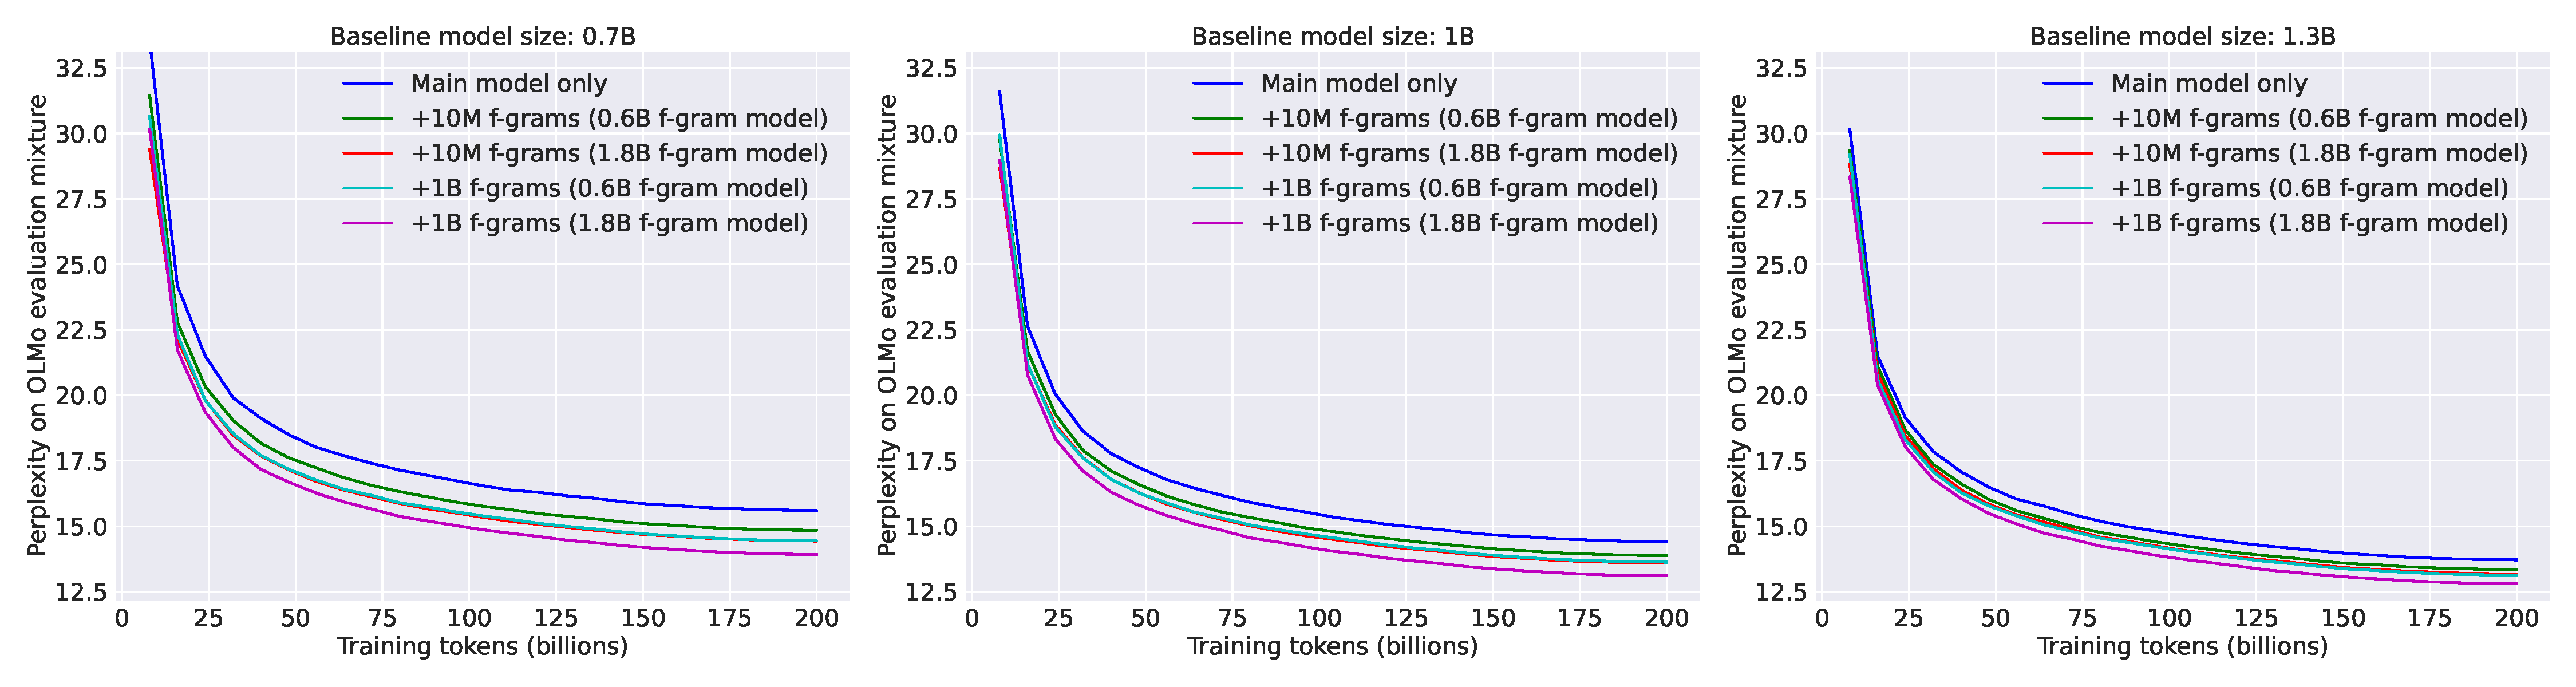
\includegraphics[width=1.0\linewidth]{figs/olmo_all_loss_curves.pdf}
    \caption{Average perplexity on the OLMo evaluation mixture throughout training. Models with \SCONE enabled converge later, indicating stronger capacity, and achieve better perplexity.}
    \label{fig:olmo_all_training_curves}
\end{figure}

\paragraph{Training Curves.} \Cref{fig:olmo_all_training_curves} shows the evaluation perplexity curves for OLMo-0.7B, OLMo-1B, and OLMo-1.3B throughout training. The curves indicate that models trained with \SCONE converge more slowly, suggesting that \SCONE effectively increases model capacity. Furthermore, both increasing the number of f-grams and enlarging the $\Afgram$ model size enhance model capacity.


\paragraph{Perplexity Evaluation.} 

\begin{table*}[htbp]
\caption{\SCONE consistently improves perplexity (lower is better) across all evaluation corpora. We train three baseline models with sizes of 1B, 1.3B, and 1.9B parameters. For the 1B and 1.3B baseline models, we apply \SCONE using four different configurations and present the results directly below each corresponding baseline.}
\label{table:olmo_breakdown}
\centering
\setlength{\tabcolsep}{5pt}
\resizebox{1.0\linewidth}{!}{
\begin{tabular}{c|ccccccccccc|c}
\toprule
 \textbf{Model size} & \textbf{c4-en} & \textbf{books} & \textbf{common-crawl} & \textbf{pes2o} & \textbf{reddit} & \textbf{stack} & \textbf{wiki} & \textbf{ice} & \textbf{m2de-s2orc} & \textbf{pile} & \textbf{wikitext-103} & \textbf{Average} \\
 \midrule
% \midrule
  \textbf{1B baseline} &  16.813 &  21.570 & 16.752 & 11.682 & 22.612 &  3.360 & 14.453  & 15.281  &  27.900 & 10.429   & 16.053  & 16.082 \\
%  \midrule
 +10M $\Vfgram$ (0.6B $\Afgram$) &  16.087 &  20.963 & 16.039 & 11.270 & 21.797 &  3.274 & 13.777  & 14.979  &  26.361 & 10.128   & 15.371  & 15.459 \\
%   \midrule
  +10M $\Vfgram$ (1.8B $\Afgram$) &  15.727 &  20.429 & 15.473 & 11.124 & 21.388 &  3.231 & 13.454  & 14.709  &  25.785 & 9.956   & 15.104  & 15.125 \\
%  \midrule
  +1B $\Vfgram$ (0.6B $\Afgram$) &   15.846 &  20.593 & 15.684 & 11.071 & 21.411 &  3.213 & 13.543  & 14.702  &  26.026 & 9.889   & 15.077  & 15.187 \\
%  \midrule
  +1B $\Vfgram$ (1.8B $\Afgram$) &  15.158 &  19.680 & 14.857 & 10.761 & 20.757 &  3.133 & 12.964  & 14.220  &  24.958 & 9.553   & 14.354  & 14.581 \\
% \midrule
 \midrule
  \textbf{1.3B baseline} & 15.994 &  20.157 & 15.921 & 11.148 & 21.634 &  3.248 & 13.721  & 14.651  &  26.583 & 9.927   & 15.143  & 15.284 \\
%  \midrule
  +10M $\Vfgram$ (0.6B $\Afgram$) &  15.509 &  19.816 & 15.407 & 10.887 & 21.022 &  3.192 & 13.260  & 14.372  &  25.450 & 9.757   & 14.616  & 14.844 \\
%  \midrule
  +10M $\Vfgram$ (1.8B $\Afgram$) & 15.193 &  19.587 & 14.995 & 10.795 & 20.735 &  3.171 & 13.071  & 14.272  &  25.258 & 9.674   & 14.438  & 14.654 \\
%  \midrule
  +1B $\Vfgram$ (0.6B $\Afgram$) & 15.270 &  19.510 & 15.106 & 10.707 & 20.763 &  3.139 & 13.073  & 14.177  &  25.009 & 9.546   & 14.397  & 14.609 \\
%  \midrule
  +1B $\Vfgram$ (1.8B $\Afgram$) & 14.803&  18.996 & 14.541 & 10.502 & 20.296 &  3.085 & 12.637  & 13.971  &  24.533 & 9.357   & 13.971  & 14.245 \\
%  \midrule
  \midrule
  \textbf{1.9B baseline} & 15.270 &  19.017 & 15.184 & 10.719 & 20.752 &  3.163 & 13.119  & 14.095  &  25.461 & 9.570   & 14.229  & 14.598 \\
\bottomrule
\end{tabular}
}
\end{table*}

\Cref{fig:olmo_scaling_result} presents perplexity results on the OLMo evaluation mixture\footnote{\url{https://github.com/allenai/OLMo/blob/v0.4.0/configs/official/OLMo-1B.yaml\#L90}}, which covers 11 diverse corpora, including web crawl data, literature, online forums, scientific writing, coding, and more. \Cref{table:olmo_breakdown} details the performance breakdown by corpus. Results show that increasing both $|\Vfgram|$ and the size of $\Afgram$ consistently improves performance across all datasets.

Additionally, \Cref{fig:olmo_scaling_result} reports token generation speeds measured using the vLLM framework \citep{kwon2023efficient} with a batch size of 1. Even with large $|\Vfgram|$, embedding retrieval remains efficient and is not a bottleneck for inference.

As a representative example, in the 1B model variant, the baseline achieves an average perplexity of 16.082. Setting $|\Vfgram|$ to 10M improves perplexity to 15.459 with a 0.6B $\Afgram$ model and to 15.125 with a 1.8B $\Afgram$ model—the latter outperforming the 1.3B baseline (15.284). Further increasing $|\Vfgram|$ to 1B improves perplexity to 15.187 (0.6B $\Afgram$) and 14.581 (1.8B $\Afgram$), surpassing the 1.9B baseline (14.598) while requiring only about half the FLOPS and accelerator memory at inference time.

\subsection{Apply \SCONE in Post-training}
\label{subsec:sft_qwen3}

We apply \SCONE to supervised fine-tuning of Qwen3-4B-base using the open-r1\footnote{\url{https://github.com/huggingface/open-r1}} framework and the open-r1/Mixture-of-Thoughts dataset\footnote{\url{https://huggingface.co/datasets/open-r1/Mixture-of-Thoughts}}. In this setup, Qwen3-4B serves as the main model, while Qwen3-8B-base or Qwen3-14B-base are used as the f-gram models. We set the number of f-grams to 10M and follow the training hyperparameters in open-r1. Table~\ref{tab:qwen3-results} compares the resulting \SCONE-enabled models with the Qwen3-4B baseline in terms of both accuracy and decoding latency.

\begin{table}[ht]
\centering
\small
\begin{tabularx}{\textwidth}{@{}X| c c c@{}}
\toprule
\thead{Model} &
\thead{AIME 2024\\pass@1} &
\thead{LiveCodeBench\\v4\_v5 pass@1} &
\thead{Decoding Latency\\(per-token)\\(ms)} \\
\midrule
Qwen3-4B-base & 45.3 & 30.8 & 10.05 \\
SCONE-4B (8B f-gram model) & 48.3 (+3.0) & 34.5 (+3.7) & 10.13 \\
SCONE-4B (14B f-gram model) & 51.6 (+6.3) & 36.3 (+5.5) & 10.13 \\
\bottomrule
\end{tabularx}
\caption{Performance comparison of Qwen3-4B variants on AIME 2024 and LiveCodeBench v4/v5 with decoding latency.}
\label{tab:qwen3-results}
\end{table}

These results show that SCONE consistently improves performance over the baseline, with larger f-gram models yielding greater gains, all while maintaining similar inference latency.


\subsection{Summary of Comparison on Computational Resources}
\label{subsec:compute_resources}

In \cref{tab:scone-efficiency}, we summarize the key metrics of \SCONE for the three model variants evaluated in \cref{sec:exps_dolma}. The metrics include (1) GPU memory, (2) CPU memory, (3) disk usage, and (4) FLOPS/latency for training and inference. All measurements are taken with a context length of 2048 and a batch size of 4 on a single A100 80 GB GPU. The three settings are: (1) the 1.9B baseline model, (2) SCONE 1.3B, with a 1.8B f‑gram model and 10M cached f‑gram embeddings, and (3) SCONE 1B , with a 1.8B f‑gram model and 1B cached f‑gram embeddings.

\begin{table}[ht]
\centering
\small
\begin{tabularx}{\textwidth}{@{}p{2.0cm}| c c c c c@{}}
\toprule
\thead{Model Variant} &
\thead{Peak GPU\\Memory\\(GB)} &
\thead{CPU Memory\\Overhead\\ (GB)} &
\thead{Disk\\Usage\\ (TB)} &
\thead{Decoding Latency\\(per-token)\\(ms)} &
\thead{Training FLOPS\\(per-seq.)\\($\times 10^{13}$)} \\
\midrule
1.9B baseline & 8.38 & N/A & N/A & 6.45 & $2.73$ \\
SCONE-1.3B (10M f-grams) & 5.60 & 41.76 & N/A & 4.83 & $4.94$ \\
SCONE-1B (1B f-grams) & 4.45 & N/A & 7.67 & 4.90 & $5.57$ \\
\bottomrule
\end{tabularx}
\caption{Comparison of SCONE model variants on memory, storage, latency, and compute efficiency.}
\label{tab:scone-efficiency}
\end{table}

Both memory and disk usage are reported for inference. The decoding latency is averaged over one thousand decoding steps. As shown in \cref{sec:exps_dolma}, all three models achieve similar downstream performance. Compared to the 1.9B baseline, SCONE-enabled models significantly reduce GPU memory usage and decoding latency, at the cost of increased CPU memory or disk storage. 

\section{Implementation Details}\label{sec:implementation_details}

We provide additional implementation details below. Most of our experiments are conducted on 4 8×H100 nodes, while some experiments are conducted on 2 16×A100 nodes.

While f-gram lookup is efficient for inference, it creates a bottleneck during training since at training time transformer models process all token positions in parallel. This leads to GPU idle time when fetching the longest matching f-gram on the fly. To remove this bottleneck, after we construct the set of f-grams ($\Vfgram$), we pre-scan the training sequences to tag the longest matching length for each token. During training, we can then directly retrieve the corresponding f-gram for forward computation with the $\Afgram$ model.

For the $\Afgram$ model, we use an absolute position embedding layer where the maximum position equals the longest \ngram{n} in $\Vfgram$. Within each batch, all f-grams are padded to the longest \ngram{n} length in that batch. We train all models with the bfloat16 precision.


\subsection{WebText}
\label{subsec:webtext_details}

\begin{table}[h]
    \centering
    \begin{tabular}{r|r r r}
        \toprule
        \textbf{Parameters (M)} & \textbf{d\_model} & \textbf{ffw\_size} & \textbf{n\_layers} \\
        \midrule
        128  & 1024  & 4096  & 6   \\
        204  & 1024  & 4096  & 12     \\
        491  & 1536  & 6144  & 12     \\
        759  & 1536  & 6144  & 24     \\
        589  & 1536  & 6144  & 18     \\
        1099  & 1536  & 6144  & 36    \\
        \bottomrule
    \end{tabular}
    \caption{Baseline model configurations for pre-training on WebText. For constructing the f-gram model ($\Afgram$), we vary the number of layers in the 128M, 491M, and 589M variants and discard the token embedding layer.}
    \label{tab:webtext_model_configs}
\end{table}


For pre-training on WebText \citep{openwebtext}, we follow \citet{radford2019language} and set the batch size and sequence length to 512 and 1024, respectively. \citet{radford2019language} do not specify the number of training tokens or optimizer details. We train the models for 80B tokens, roughly doubling the count in \citet{radford2018improving}. For optimization, we use AdamW \citep{loshchilov2017decoupled} with a weight decay of 0.1. Following \citet{hoffmann2022training}, we set the maximum learning rate to $2\times 10^{-4}$ and apply a cosine learning rate scheduler. We list the model configurations in \Cref{tab:webtext_model_configs}.



\subsection{OLMo Tokenized Training Corpus}
\label{subsec:dolma_details}

\begin{table}[h]
    \centering
    \begin{tabular}{r|r r r}
        \toprule
        \textbf{Parameters (M)} & \textbf{d\_model} & \textbf{ffw\_size} & \textbf{n\_layers} \\
        \midrule
         711 &  2048  &  8192  &  12   \\
        1014  &  2048   &  8192  &  18     \\
        1316  &   2048 &  8192   &  24     \\
        1920  &  2048  &  8192  &  36     \\
        \bottomrule
    \end{tabular}
    \caption{Model configurations for pre-training on the OLMo corpus. To construct the f-gram model ($\Afgram$), we use the 711M and 1920M variants, excluding the token embedding layers.}
    \label{tab:olmo_model_configs}
\end{table}


For pre-training on the OLMo tokenized training corpus, we follow the optimizer settings for the 1B variant in \citet{OLMo} \footnote{\url{https://github.com/allenai/OLMo/blob/v0.4.0/configs/official/OLMo-1B.yaml\#L40}}. All models use a sequence length of 2048. We use DeepSpeed \citep{deepspeed_repo} with ZeRO stage 1 that partitions the optimizer state across GPUs to reduce GPU memory usage. We list the model configurations in \Cref{tab:olmo_model_configs}.

